%
% management.tex
%
% Copyright The GOLDS-UFSC Contributors.
%
% GOLDS-UFSC Documentation
%
% This work is licensed under the Creative Commons Attribution-ShareAlike 4.0
% International License. To view a copy of this license,
% visit http://creativecommons.org/licenses/by-sa/4.0/.
%

%
% \brief Mission management chapter.
%
% \author Gabriel Mariano Marcelino <gabriel.mm8@gmail.com>
%
% \version 0.2.0
%
% \date 2021/07/15
%

\chapter{Mission Management} \label{ch:management}

\section{Requirements}

\begin{enumerate}
    \item The power system must be able to harvest solar energy.
    \item The power system must be able to store energy for use when GOLDS-UFSC is eclipsed.
    \item The power system must supply energy to all other modules.
    \item The data handling system must communicate with the other modules and store their data.
    \item The communications system must send a beacon signal periodically using VHF radio.
    \item The communications system must send the CubeSat telemetry using UHF radio.
    \item The communications system must be able to receive telecommands and respond to them accordingly.
    \item The attitude system must be able to perform a 1-axis stabilization of the CubeSat.
    \item GOLDS-UFSC must be able to receive and execute a shutdown telecommand, therefore ceasing all transmissions.
    \item The downlink transmissions must be done once at a time, either telemetry or beacon.
    \item The ground station must operate under the proper radio frequency communication licenses.
    \item GOLDS-UFSC must comply with international and Brazilian radio license agreements and restrictions.
    \item The team must build and operate a ground station for full communication with GOLDS-UFSC.
    \item GOLDS-UFSC must be capable of sustaining the EDC operation.
    \item The service module and payload must employ materials and components that do not compromise or damage LIT/INPE test facilities.
    \item The satellite must reenter the Earth's atmosphere within 25 years.
    \item It is recommended that the satellite be placed in an orbit up to 500 km.
\end{enumerate}

\section{Schedule}

\begin{table}[!h]
    \centering
    \begin{tabular}{cC{0.6cm}C{0.6cm}C{0.6cm}C{0.6cm}C{0.6cm}C{0.6cm}C{0.6cm}C{0.6cm}C{0.6cm}C{0.6cm}C{0.6cm}C{0.6cm}C{0.6cm}C{0.6cm}}
        \toprule[1.5pt]
        \multirow{4}{*}{\textbf{Activity}} & \multicolumn{14}{c}{\textbf{Month}} \\
                                           & Nov & Dez & Jan & Feb & Mar & Apr & May & Jun & Jul & Aug & Sep & Oct & Nov & Dez \\
                                           & 22  & 22  & 23  & 23  & 23  & 23  & 23  & 23  & 23  & 23  & 23  & 23  & 23  & 23 \\
        \midrule
        1                                  & \fc & \fc & \fc & \fc & \fc & \fc &     &     &     &     &     &     &     &     \\
        2                                  & \fc & \fc & \fc & \fc & \fc & \fc &     &     &     &     &     &     &     &     \\
        3                                  &     &     & \fc & \fc & \fc & \fc & \fc & \fc & \fc & \fc & \fc &     &     &     \\
        4                                  &     &     & \fc & \fc & \fc & \fc & \fc & \fc &     &     &     &     &     &     \\
        5                                  &     &     &     &     &     & \fc & \fc & \fc & \fc & \fc & \fc & \fc &     &     \\
        6                                  &     &     &     &     &     &     & \fc & \fc & \fc & \fc & \fc & \fc & \fc &     \\
        7                                  &     &     &     &     &     &     &     &     &     & \fc & \fc & \fc &     &     \\
        8                                  &     &     &     &     &     &     &     &     &     & \fc & \fc & \fc & \fc &     \\
        9                                  &     &     &     &     &     &     &     &     &     &     & \fc & \fc & \fc & \fc \\
        10                                 &     &     &     &     &     &     &     &     &     &     &     & \fc & \fc &     \\
        11                                 &     &     &     &     &     &     &     &     &     &     &     & \fc & \fc &     \\
        12                                 &     &     &     &     &     &     &     &     &     &     &     &     & \fc &     \\
        13                                 &     &     &     &     &     &     &     &     &     &     & \fc & \fc & \fc & \fc \\
        14                                 &     &     &     &     &     &     &     &     &     &     &     &     & \fc & \fc \\
        \bottomrule[1.5pt]
    \end{tabular}
    \caption{Mission schedule.}
    \label{tab:mission-schedule}
\end{table}

Each activity of \autoref{tab:mission-schedule} is described below:

\begin{enumerate}
    \item Integration of the engineering model in SpaceLab UFSC.
    \item Preparation and suitability of the ground segment.
    \item Verification and validation of the engineering model.
    \item Integration and verification with data collection platforms.
    \item Verification and validation tests of Engineering Model compatibility with EMMN in the INPE / CRN in Natal.
    \item Verification and validation of the flight model.
    \item Environmental tests at the Integration and Testing Laboratory (LIT/INPE).
    \item Flight model acceptance and ground segment review.
    \item Ground segment delivery.
    \item Flight model delivery.
\end{enumerate}

\section{Product Tree}


\begin{figure}[!ht]
    \begin{center}
        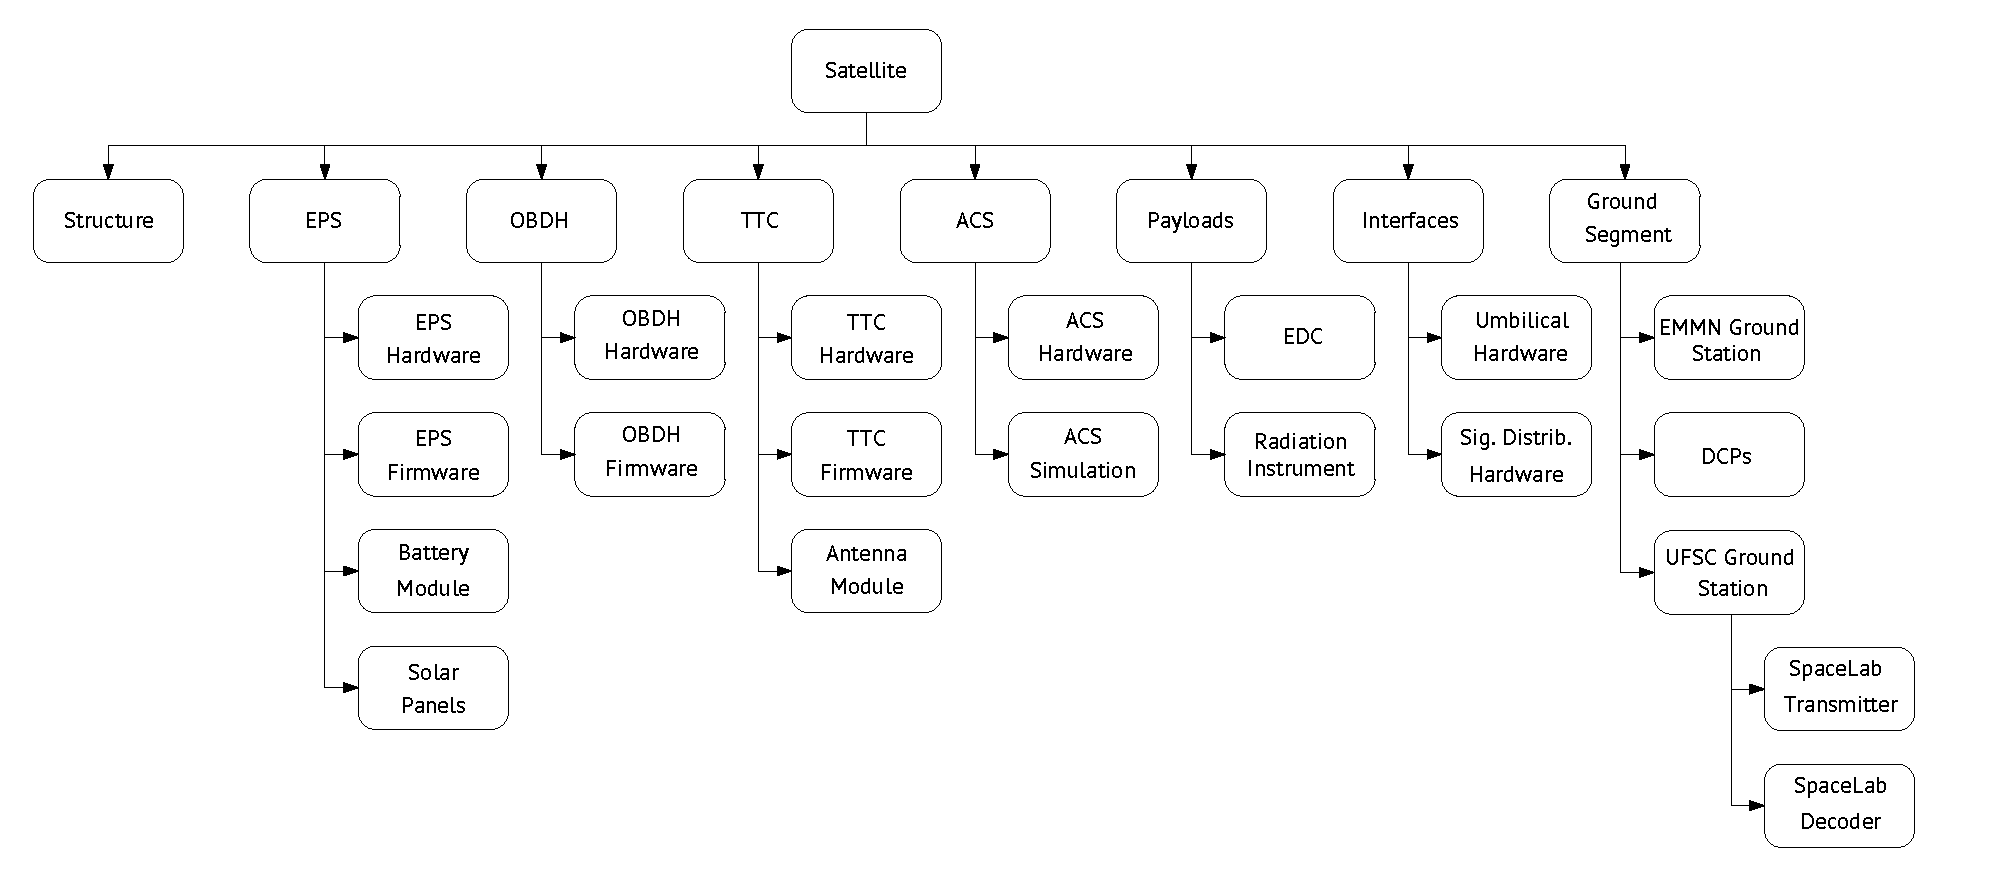
\includegraphics[width=\textwidth]{figures/product-tree.pdf}
        \caption{Product tree of the satellite.}
        \label{fig:product-tree}
    \end{center}
\end{figure}

\subsection{Working Breakdown Structure}

The Working Breaking Structure (WBS\nomenclature{\textbf{WBS}}{\textit{Working Breakdown Structure.}}) is presented as a diagram in \autoref{fig:wbs}. The WBS is divided into work packages (WP\nomenclature{\textbf{WP}}{\textit{Work Package.}}) as can be seen in the diagram. The description of each WP is detailed below.

\begin{figure}[!ht]
    \begin{center}
        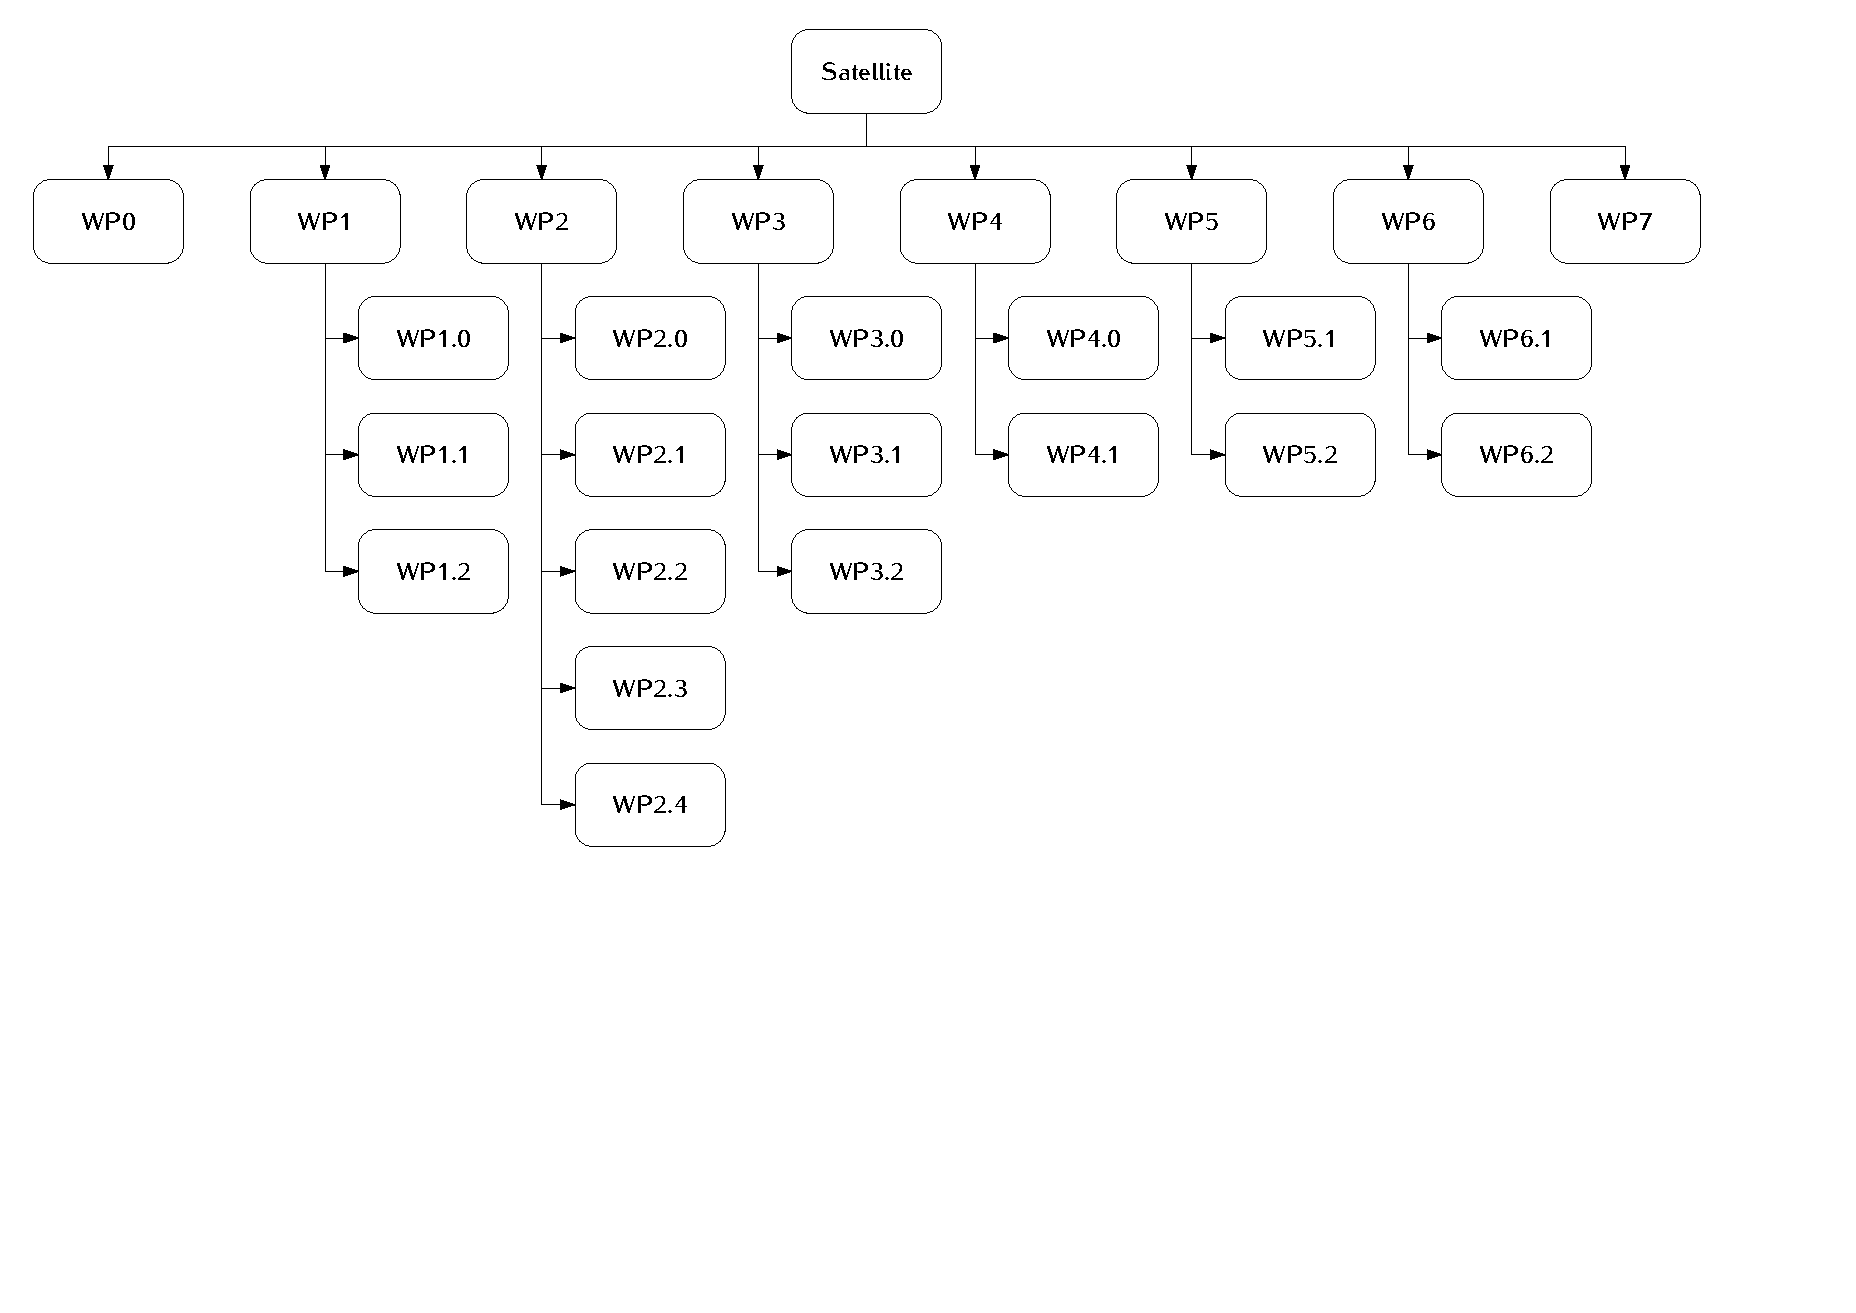
\includegraphics[width=\textwidth]{figures/wbs.pdf}
        \caption{WBS diagram.}
        \label{fig:wbs}
    \end{center}
\end{figure}

\begin{itemize}
    \item \textbf{WP0}: Management and preparation.
    \item \textbf{WP1}: Architecture study and specification.
        \begin{itemize}
            \item \textbf{WP1.0}: Operation scenario definition.
            \item \textbf{WP1.1}: Architecture definition.
            \item \textbf{WP1.2}: Requirements definition.
        \end{itemize}
    \item \textbf{WP2}: Engineering and flight models definition
        \begin{itemize}
            \item \textbf{WP2.0}: Application design.
            \item \textbf{WP2.1}: Platform design.
            \item \textbf{WP2.2}: Application implementation.
            \item \textbf{WP2.3}: Platform implementation.
            \item \textbf{WP2.4}: Decoder implementation (EGSE).
        \end{itemize}
    \item \textbf{WP3}: Engineering model integration.
        \begin{itemize}
            \item \textbf{WP3.0}: Subsystems integration and tests.
            \item \textbf{WP3.1}: Engineering model satellite integration.
            \item \textbf{WP3.2}: Integration and tests with decoder.
        \end{itemize}
    \item \textbf{WP4}: Engineering model validation.
        \begin{itemize}
            \item \textbf{WP4.0}: Validation scenarios specification.
            \item \textbf{WP4.1}: Project validation.
        \end{itemize}
    \item \textbf{WP5}: Fligth model integration.
        \begin{itemize}
            \item \textbf{WP5.0}: Subsystems integration and tests.
            \item \textbf{WP5.1}: Fligth model satellite integration.
        \end{itemize}
    \item \textbf{WP6}: Fligth model validation.
        \begin{itemize}
            \item \textbf{WP6.0}: Validation scenarios specification.
            \item \textbf{WP6.1}: Project validation.
        \end{itemize}
    \item \textbf{WP7}: Evaluation and dissemination.
\end{itemize}
